\documentclass{article}
\usepackage{graphicx}
\usepackage[margin=1.5cm]{geometry}
\usepackage{amsmath}

\begin{document}

\title{Wednesday Reading Assessment: Unit 7, Power and Conservation of Energy}
\author{Prof. Jordan C. Hanson}

\maketitle

\section{Memory Bank}

\begin{itemize}
\item $W = \vec{F} \cdot \Delta \vec{x}$ ... Definition of work, Joules.
\item $P = dW/dt$ ... Definition of power, Watts.
\item $U = mg\Delta y$ ... Gravitational potential energy.
\end{itemize}

\section{Work and Power}

\begin{enumerate}
\item An 80-kg army trainee does 10 pull-ups in 10 seconds.  Assume the trainee raises his center of mass by $\Delta t = 0.6$ meters.  How much average power do the trainee’s muscles supply moving his body?
\begin{figure}[ht]
\centering
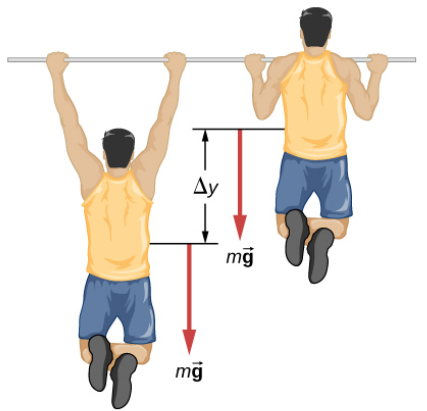
\includegraphics[width=0.4\textwidth]{pullup.png}
\caption{\label{fig:work} An army trainee does pullups at a certain rate.}
\end{figure}
\item The unit of \textit{horsepower} is sometimes used to describe engines.  One horsepower is equal to 746 Watts.  (a) How many Watts can a 200 horsepower engine produce? (b) Another engine provides $3\times 10^6$ J of work in 1 hour.  How many horsepower does it have?
\end{enumerate}
\end{document}